% Atom, description, circuit, SKETCH
\appendix
\section{SKETCH code and circuit diagrams for atoms}

We now describe the atoms in Table~\ref{tab:templates} in further detail by
providing circuit diagrams for each and SKETCH code for the atom templates.
Table~\ref{tab:sketch_constructs} summarizes the SKETCH notation we use in this
section.

\begin{table}
  \begin{scriptsize}
  \begin{tabular}{p{0.3\columnwidth}p{0.7\columnwidth}}
  SKETCH construct & Description \\
  \hline
  MuxN(a1, a2, \dots, aN) & \pbox{0.7\columnwidth}{N-to-1 multiplexer with enable bit.\\If enabled, return one of a1, a2, \dots aN.\\If disabled, return 0.}\\
  Opt(a)        & Return a or 0. \\
  rel\_op(x, y) & Return one of $x < y$, $x > y$, $x != y$, $x == y$.\\
  C() & Return an integer constant in the range [0, 31].\footnote{We restrict constants to 5 bits because all constants in our dataplane algorithms are under 32. Larger ranges increase synthesis time.} \\
  state\_1, state\_2 & State variables \\
  pkt\_1, pkt\_2 & Packet fields \\
  \end{tabular}
  \end{scriptsize}
  \caption{SKETCH notation used in atom templates}
  \label{tab:sketch_constructs}
\end{table}

\onecolumn

\begin{scriptsize}
\begin{longtable}{|p{0.1\textwidth}|p{0.5\textwidth}|p{0.35\textwidth}|p{0.03\textwidth}|}
      \hline
      Atom & Circuit & SKETCH code & Circuit depth \\

\hline
Write &
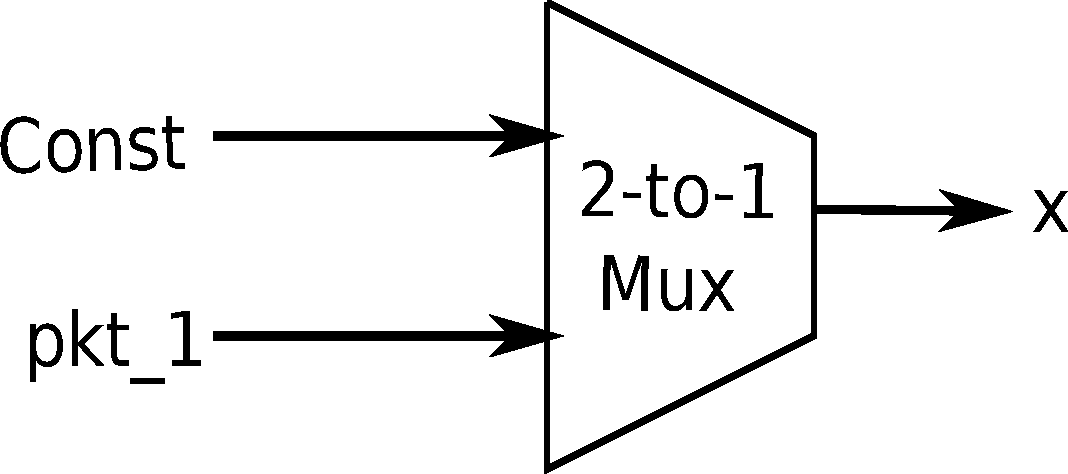
\includegraphics[width=0.2\textwidth]{rw.pdf} &
{\begin{lstlisting}[style=customctable]
  state_1 = Mux2(pkt_1, C());
 \end{lstlisting}} &
1 \\

\hline
ReadAddWrite (RAW) &
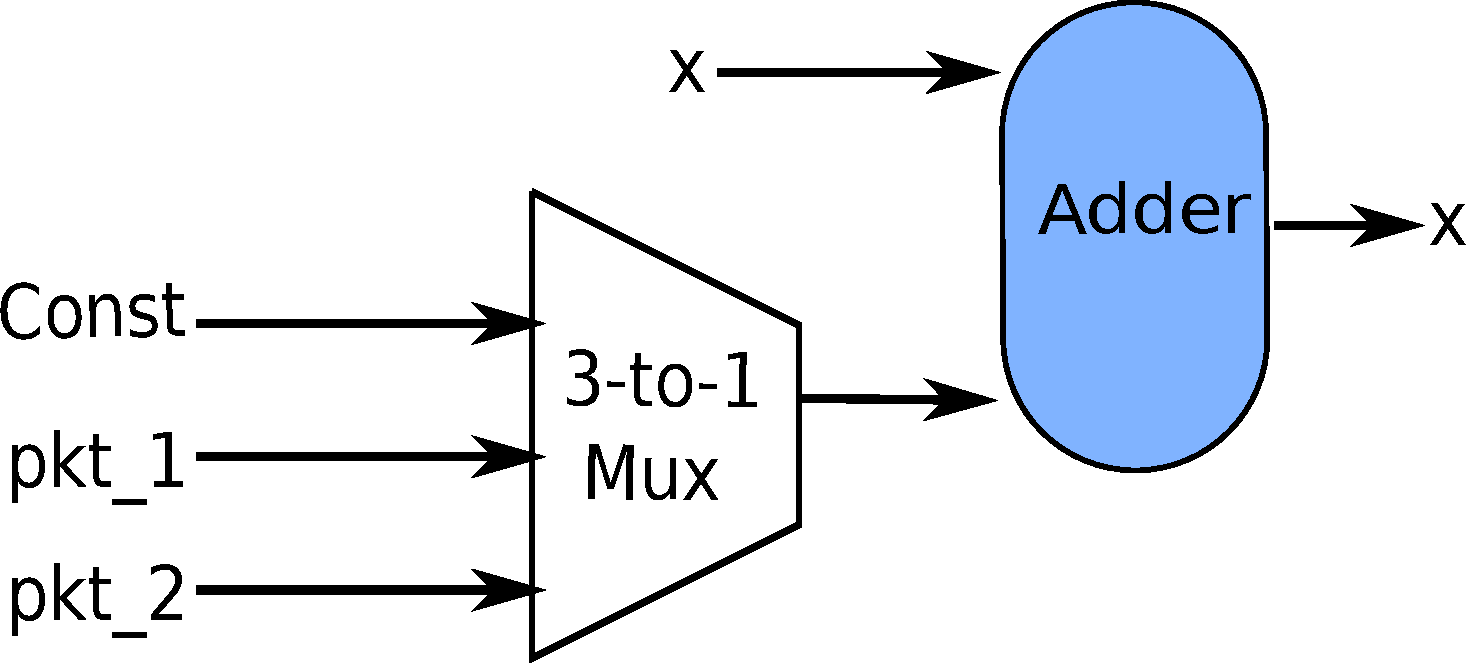
\includegraphics[width=0.3\textwidth]{raw.pdf} &
{\begin{lstlisting}[style=customctable]
 state_1 = Opt(state_1)
           + Mux2(pkt_1, C());
 \end{lstlisting}} &
2\\

\hline
\pbox{0.1\textwidth}
{Predicated\\
ReadAddWrite (PRAW)} &
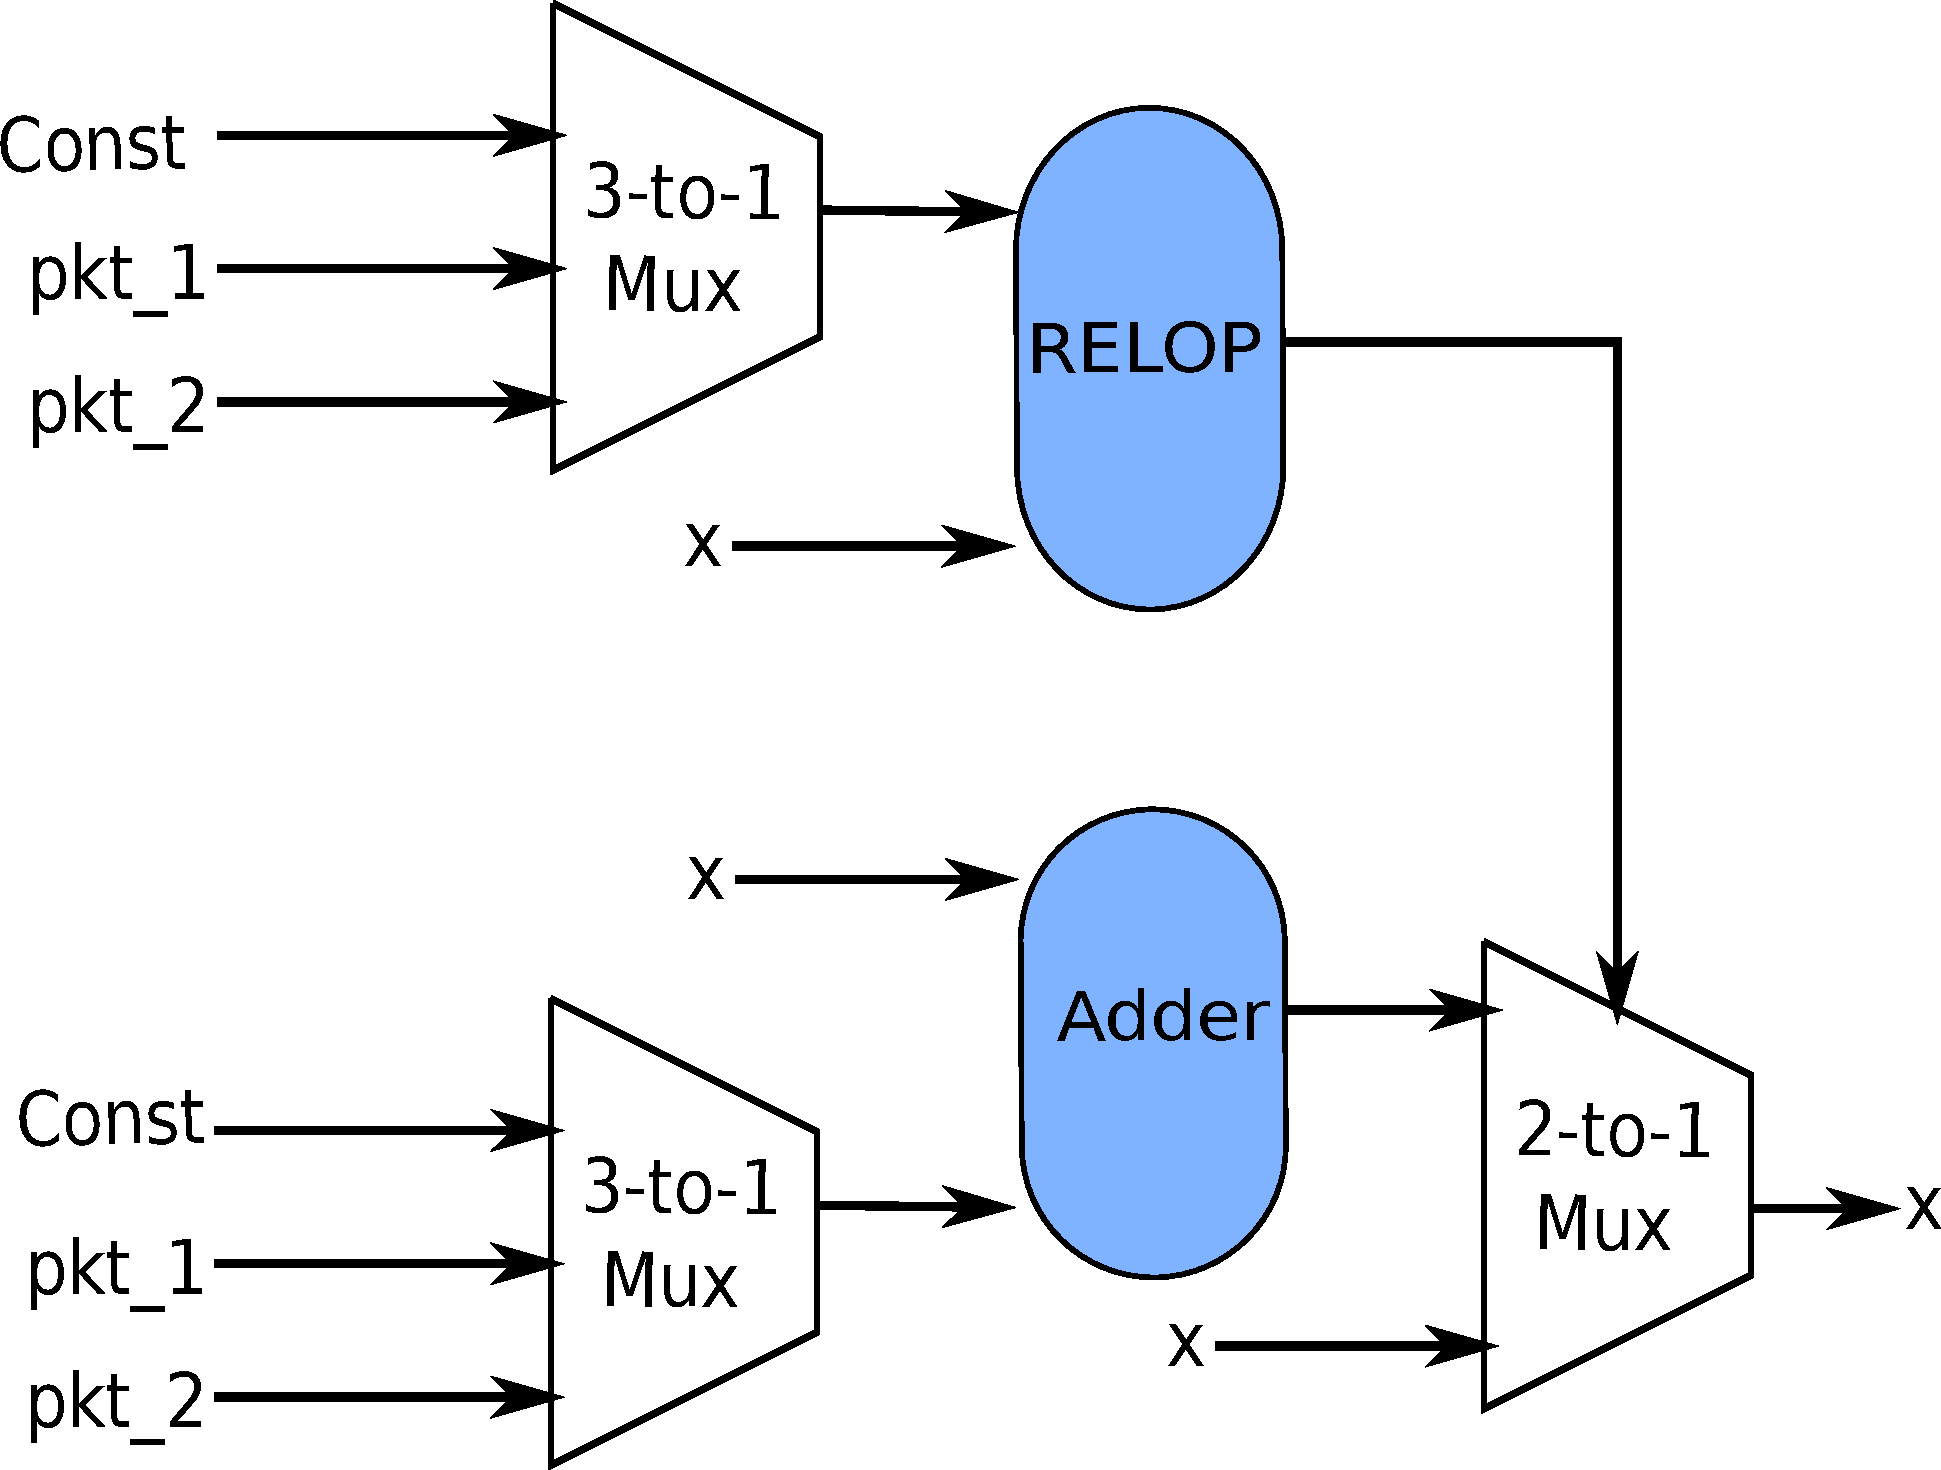
\includegraphics[width=0.4\textwidth]{pred_raw.pdf}  &
{\begin{lstlisting}[style=customctable]
if (rel_op(Opt(state_1),
           Mux3(pkt_1, pkt_2, C()))) {
  state_1 = Opt(state_1)
            + Mux3(pkt_1, pkt_2, C());
}
\end{lstlisting}} &
3\\

\hline
\pbox{0.1\textwidth}
{If-Else\\
ReadAddWrite (IfElseRAW)} &
  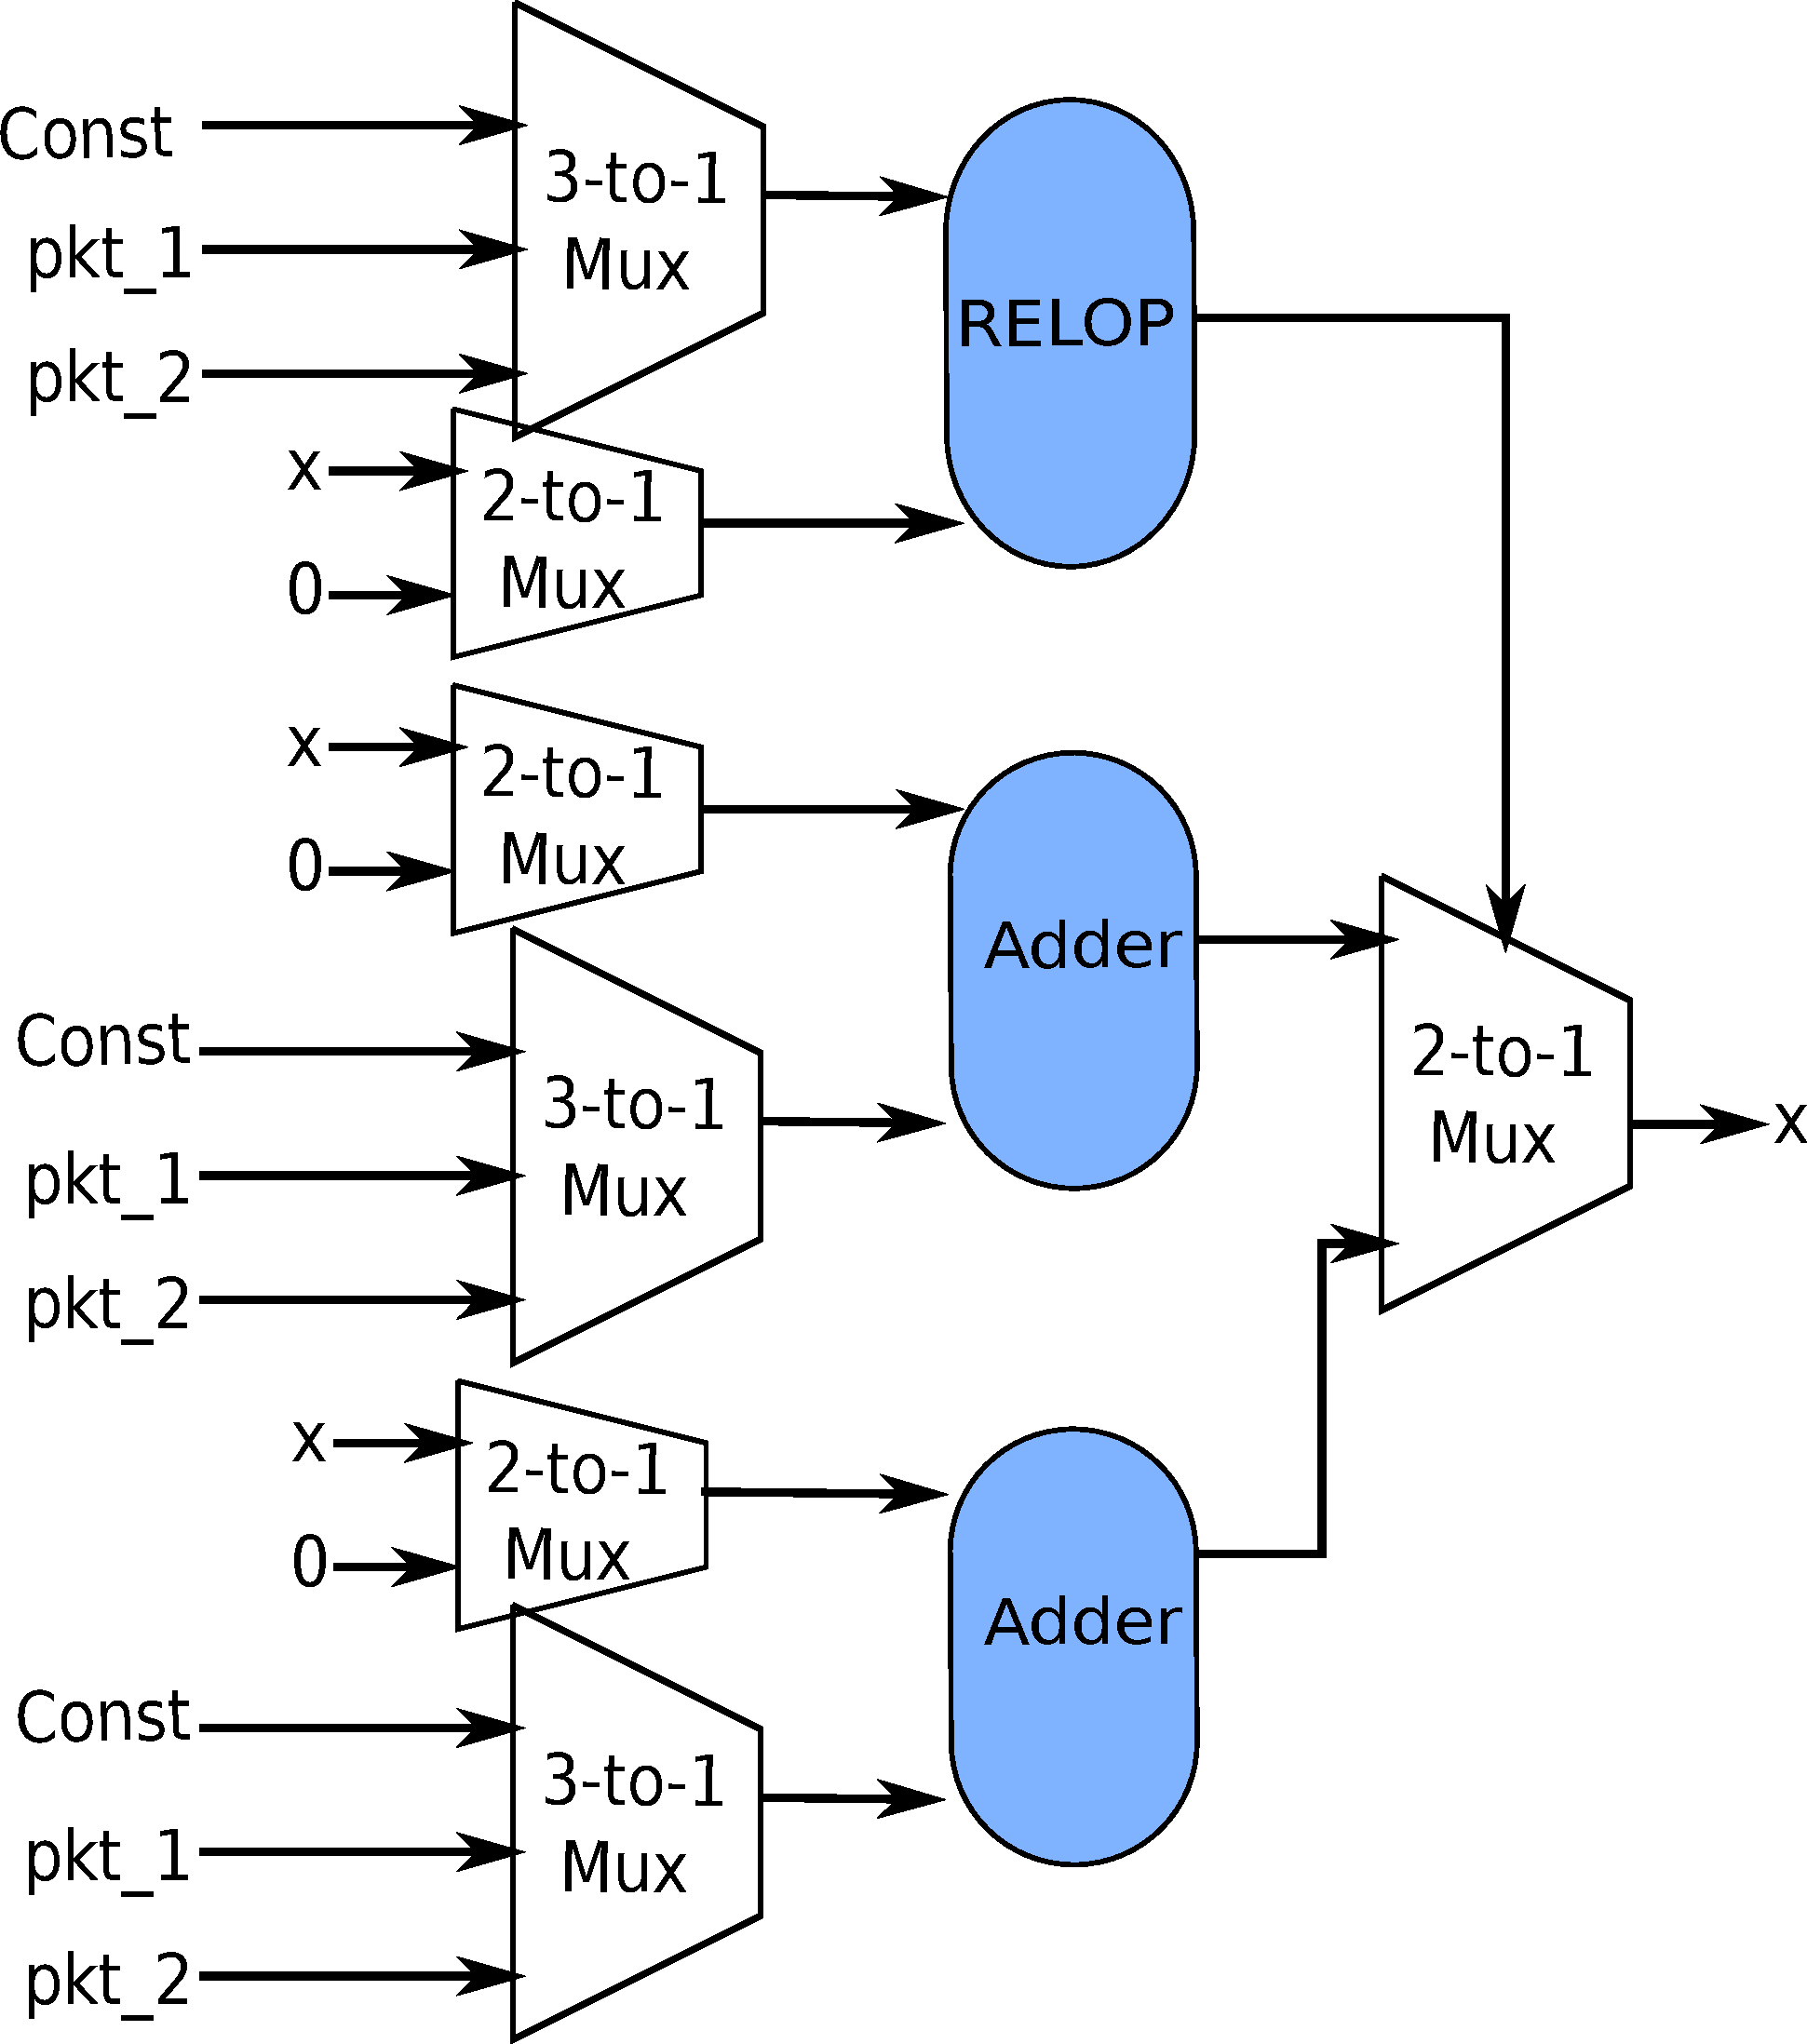
\includegraphics[width=0.4\textwidth]{if_else.pdf} &
{\begin{lstlisting}[style=customctable]
if (rel_op(Opt(state_1),
           Mux3(pkt_1, pkt_2, C()))) {
  state_1 = Opt(state_1)
            + Mux3(pkt_1, pkt_2, C());
} else {
  state_1 = Opt(state_1)
            + Mux3(pkt_1, pkt_2, C());
}
\end{lstlisting}} &
3\\

\hline
\pbox{0.1\textwidth}
{Subtract (Sub)} &
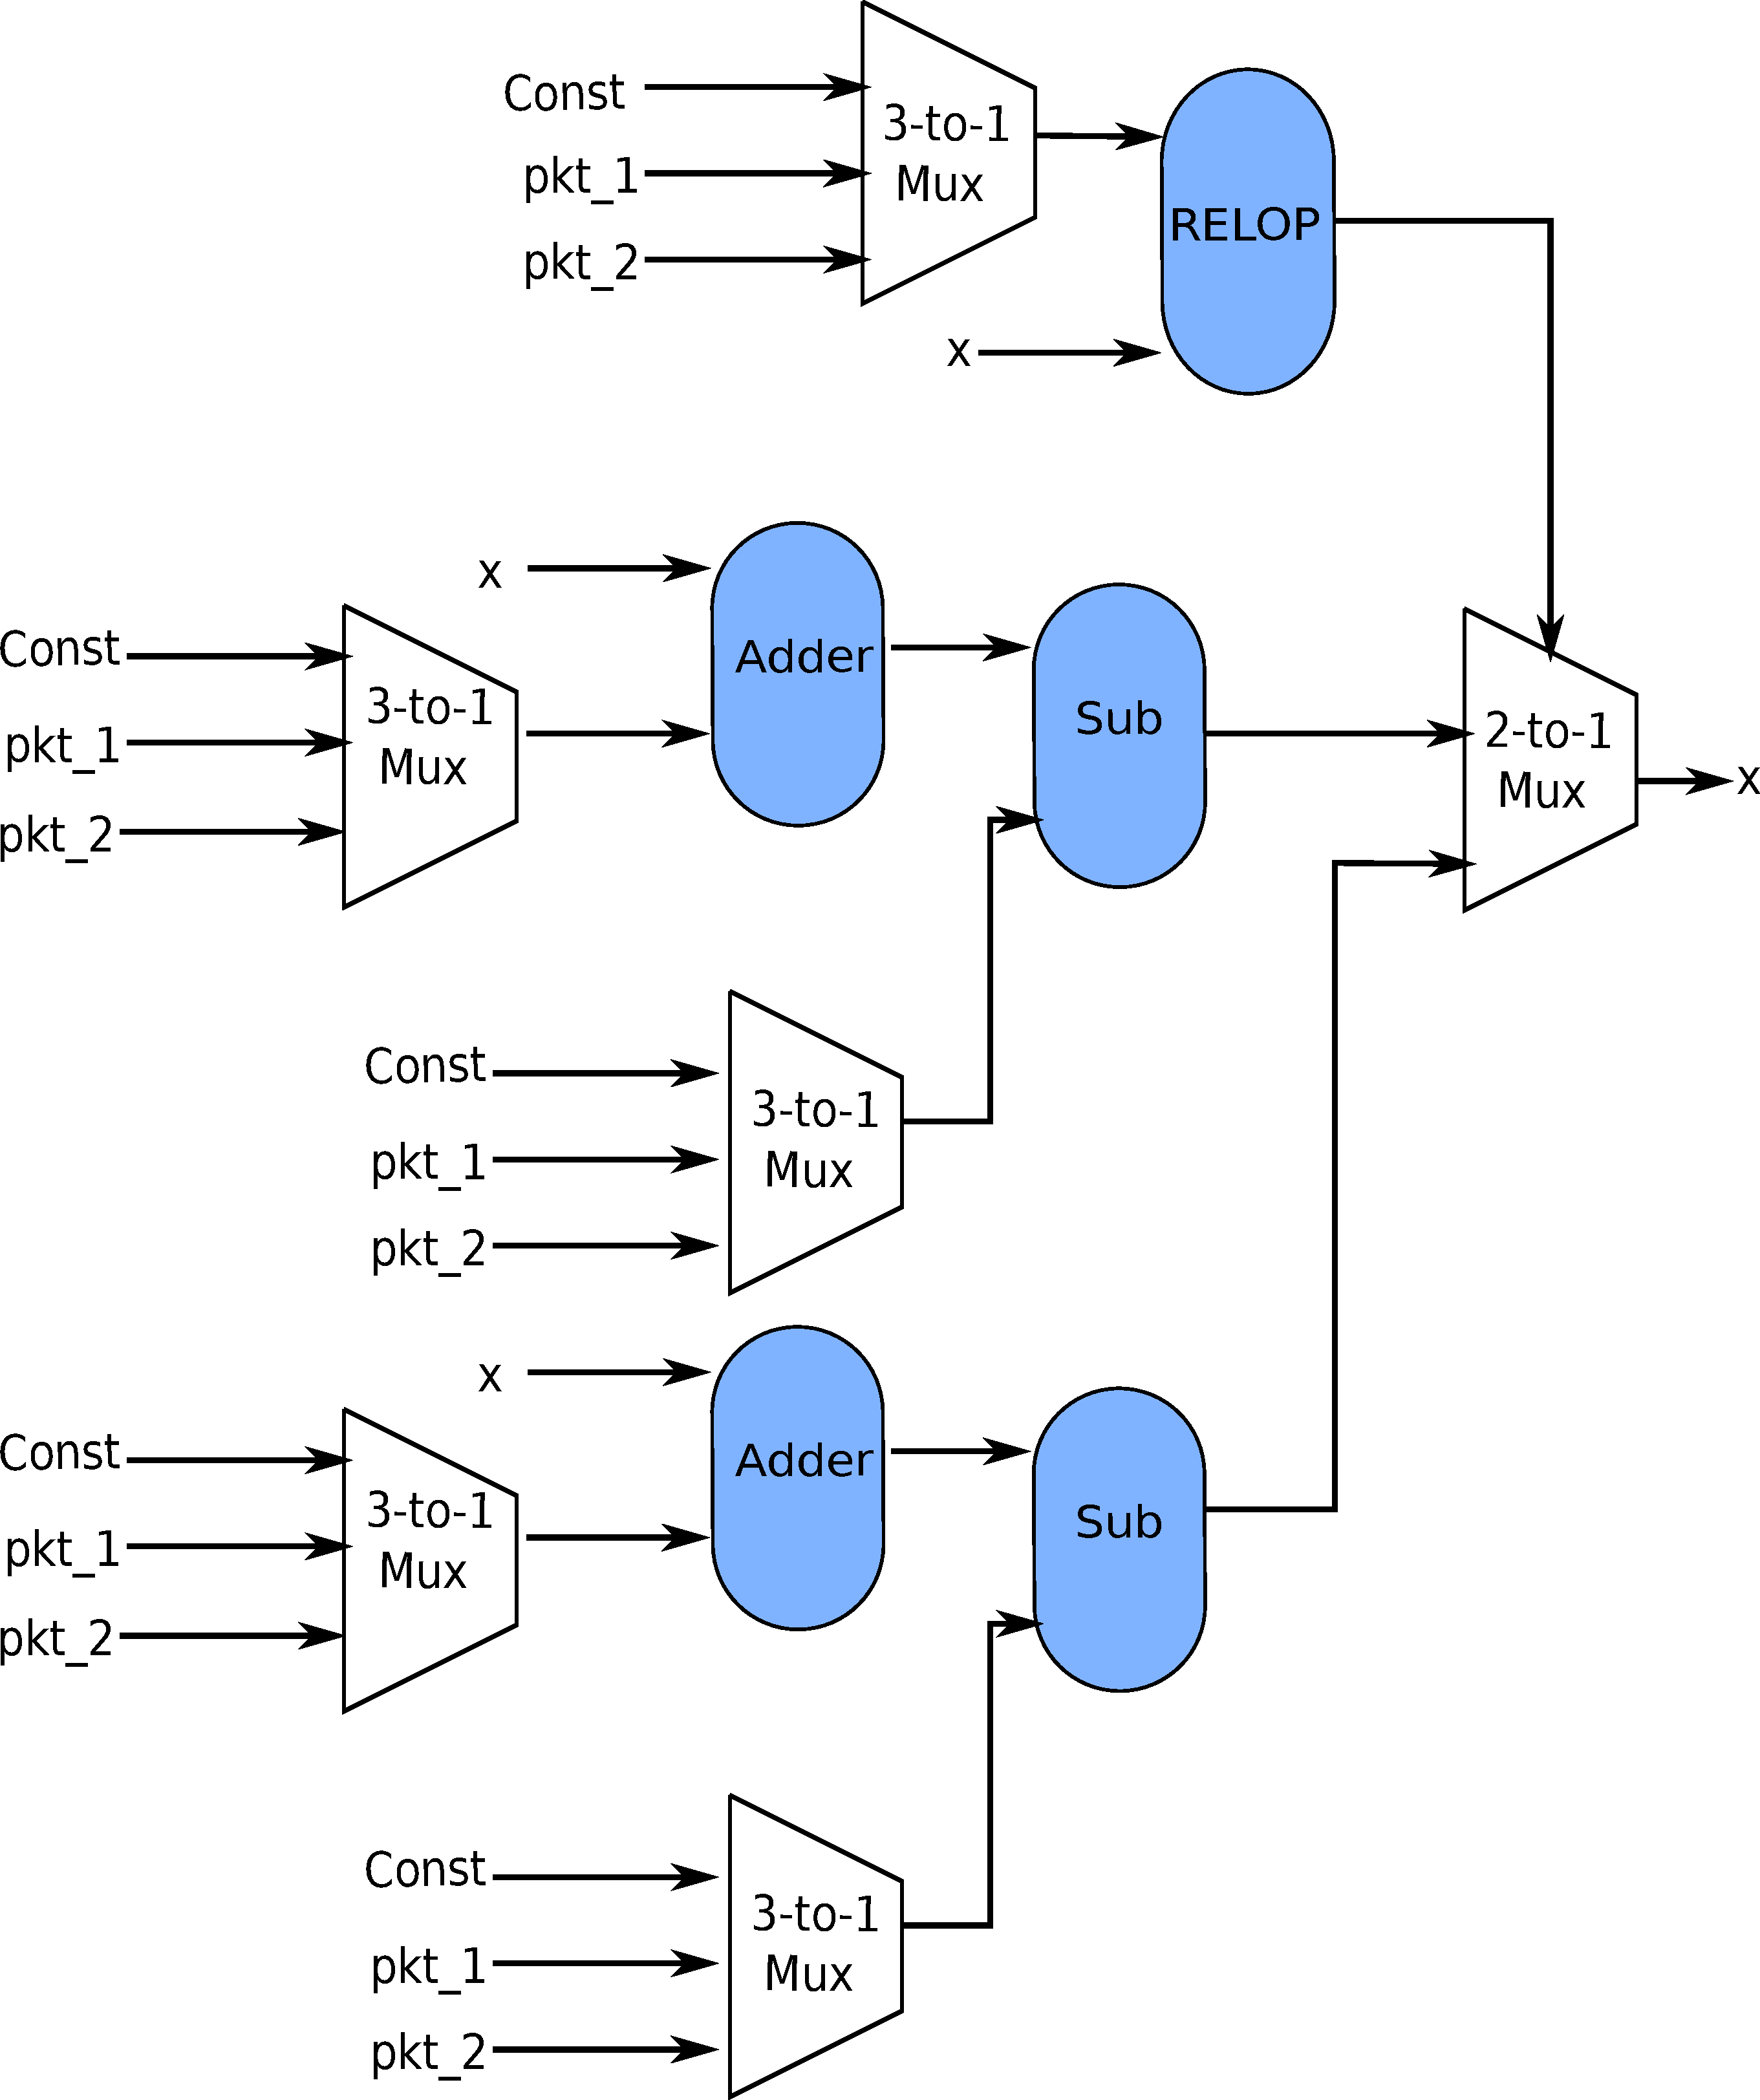
\includegraphics[width=0.45\textwidth]{sub.pdf} &
{\begin{lstlisting}[style=customctable]
if (rel_op(Opt(state_1),
           Mux3(pkt_1, pkt_2, C()))) {
  state_1 = Opt(state_1)
            + Mux3(pkt_1, pkt_2, C())
            - Mux3(pkt_1, pkt_2, C());
} else {
  state_1 = Opt(state_1)
            + Mux3(pkt_1, pkt_2, C())
            - Mux3(pkt_1, pkt_2, C());
}
\end{lstlisting}}&
4 \\

\hline
  \end{longtable}
  \end{scriptsize}

\twocolumn
